\documentclass{standalone}
\usepackage{graphicx}
\usepackage{tikz}
\usetikzlibrary{calc}
\usepackage{xcolor}
\begin{document}
\def\darkgreen{green!60!black}
\def\darkgrey{gray!80!black}
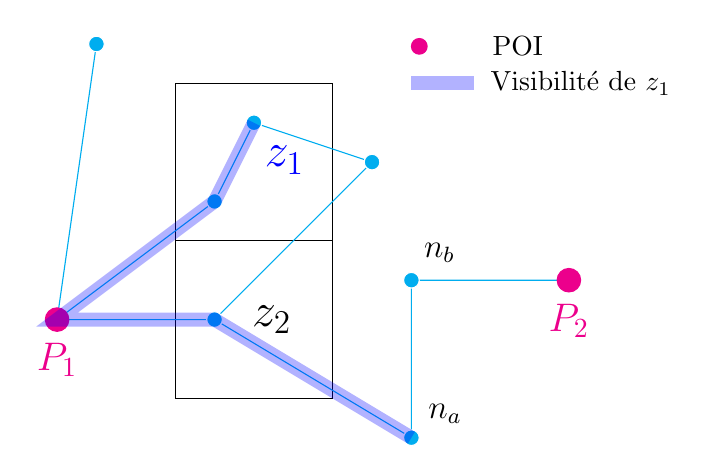
\begin{tikzpicture}[
    shift={(0,0)},
    dashblue/.style={dash pattern=on 4pt off 2pt, draw=blue, very thick},
    dashgreen/.style={dash pattern=on 4pt off 2pt, draw=\darkgreen, very thick},
    POI/.style={fill=magenta, draw=magenta},
    smallcircle/.style={circle, draw=white, fill=cyan, inner sep=2pt},
    bluehighlight/.style={draw=blue, line width=5pt,opacity=0.3},
]

% tiles
\draw[\darkgrey] (0,0) -- (2,0) -- (2,2) -- (0,2) -- (0,0);
\draw[\darkgrey] (0,0) -- (2,0) -- (2,-2) -- (0,-2) -- (0,0);

% noeuds
\coordinate [label={[blue,label distance=5]-85:\LARGE \(z_{1}\)}] (P1) at (2/2,3/2);
\coordinate [label={[\darkgreen,label distance=10]0:\LARGE \(z_{2}\)}] (P2) at (1/2,-2/2);
\coordinate [label={[magenta,label distance=5]-90:\Large \(P_{1}\)}] (P3) at (-3/2,-2/2);
\coordinate [label={[magenta,label distance=5]-90:\Large \(P_{2}\)}] (P4) at (10/2,-1/2);
\coordinate (P5) at (1/2,1/2);
\coordinate (P6) at (5/2,2/2);
\coordinate [label={[label distance=3]30:\large \(n_{a}\)}] (P7) at (6/2,-5/2);
\coordinate [label={[label distance=3]70:\large \(n_{b}\)}] (P8) at (6/2,-1/2);
\coordinate (P9) at (-2/2,5/2);

% dessiner graphe
\draw[cyan] (P2)--(P3)--(P9)--(P3)--(P5)--(P1)--(P6)--(P2)--(P7)--(P8)--(P4);
\foreach \P in {P1,P2,P3,P4,P5,P6,P7,P8,P9}{
  \node[smallcircle] at (\P) {};
}
% POI
\node[POI, circle, inner sep=3pt] at (P3) {};
\node[POI, circle, inner sep=3pt] at (P4) {};

% dessiner la visi
\draw[bluehighlight] (P1)--(P5)--(P3)--(P2)--(P7);

% legende
\begin{scope}[shift={(3,2)}]
  \node[POI, circle, inner sep=2pt] at (0.1,0.47) {};
  \node at (1.35,0.47) {POI};
  \draw[bluehighlight] (0,0) -- (0.8,0);
  \node at (2.15,0) {Visibilité de $z_1$};
  % \draw[dashgreen] (0,-0.5) -- (0.8,-0.5) node[right=2pt] {PCC de $z_2$};
\end{scope}

\end{tikzpicture}
\end{document}
